\PassOptionsToPackage{unicode=true}{hyperref} % options for packages loaded elsewhere
\PassOptionsToPackage{hyphens}{url}
%
\documentclass[]{article}
\usepackage{lmodern}
\usepackage{amssymb,amsmath}
\usepackage{ifxetex,ifluatex}
\usepackage{fixltx2e} % provides \textsubscript
\ifnum 0\ifxetex 1\fi\ifluatex 1\fi=0 % if pdftex
  \usepackage[T1]{fontenc}
  \usepackage[utf8]{inputenc}
  \usepackage{textcomp} % provides euro and other symbols
\else % if luatex or xelatex
  \usepackage{unicode-math}
  \defaultfontfeatures{Ligatures=TeX,Scale=MatchLowercase}
\fi
% use upquote if available, for straight quotes in verbatim environments
\IfFileExists{upquote.sty}{\usepackage{upquote}}{}
% use microtype if available
\IfFileExists{microtype.sty}{%
\usepackage[]{microtype}
\UseMicrotypeSet[protrusion]{basicmath} % disable protrusion for tt fonts
}{}
\IfFileExists{parskip.sty}{%
\usepackage{parskip}
}{% else
\setlength{\parindent}{0pt}
\setlength{\parskip}{6pt plus 2pt minus 1pt}
}
\usepackage{hyperref}
\hypersetup{
            pdftitle={Model Questions},
            pdfauthor={Thiyanga Talagala},
            pdfborder={0 0 0},
            breaklinks=true}
\urlstyle{same}  % don't use monospace font for urls
\usepackage[margin=1in]{geometry}
\usepackage{color}
\usepackage{fancyvrb}
\newcommand{\VerbBar}{|}
\newcommand{\VERB}{\Verb[commandchars=\\\{\}]}
\DefineVerbatimEnvironment{Highlighting}{Verbatim}{commandchars=\\\{\}}
% Add ',fontsize=\small' for more characters per line
\usepackage{framed}
\definecolor{shadecolor}{RGB}{248,248,248}
\newenvironment{Shaded}{\begin{snugshade}}{\end{snugshade}}
\newcommand{\AlertTok}[1]{\textcolor[rgb]{0.94,0.16,0.16}{#1}}
\newcommand{\AnnotationTok}[1]{\textcolor[rgb]{0.56,0.35,0.01}{\textbf{\textit{#1}}}}
\newcommand{\AttributeTok}[1]{\textcolor[rgb]{0.77,0.63,0.00}{#1}}
\newcommand{\BaseNTok}[1]{\textcolor[rgb]{0.00,0.00,0.81}{#1}}
\newcommand{\BuiltInTok}[1]{#1}
\newcommand{\CharTok}[1]{\textcolor[rgb]{0.31,0.60,0.02}{#1}}
\newcommand{\CommentTok}[1]{\textcolor[rgb]{0.56,0.35,0.01}{\textit{#1}}}
\newcommand{\CommentVarTok}[1]{\textcolor[rgb]{0.56,0.35,0.01}{\textbf{\textit{#1}}}}
\newcommand{\ConstantTok}[1]{\textcolor[rgb]{0.00,0.00,0.00}{#1}}
\newcommand{\ControlFlowTok}[1]{\textcolor[rgb]{0.13,0.29,0.53}{\textbf{#1}}}
\newcommand{\DataTypeTok}[1]{\textcolor[rgb]{0.13,0.29,0.53}{#1}}
\newcommand{\DecValTok}[1]{\textcolor[rgb]{0.00,0.00,0.81}{#1}}
\newcommand{\DocumentationTok}[1]{\textcolor[rgb]{0.56,0.35,0.01}{\textbf{\textit{#1}}}}
\newcommand{\ErrorTok}[1]{\textcolor[rgb]{0.64,0.00,0.00}{\textbf{#1}}}
\newcommand{\ExtensionTok}[1]{#1}
\newcommand{\FloatTok}[1]{\textcolor[rgb]{0.00,0.00,0.81}{#1}}
\newcommand{\FunctionTok}[1]{\textcolor[rgb]{0.00,0.00,0.00}{#1}}
\newcommand{\ImportTok}[1]{#1}
\newcommand{\InformationTok}[1]{\textcolor[rgb]{0.56,0.35,0.01}{\textbf{\textit{#1}}}}
\newcommand{\KeywordTok}[1]{\textcolor[rgb]{0.13,0.29,0.53}{\textbf{#1}}}
\newcommand{\NormalTok}[1]{#1}
\newcommand{\OperatorTok}[1]{\textcolor[rgb]{0.81,0.36,0.00}{\textbf{#1}}}
\newcommand{\OtherTok}[1]{\textcolor[rgb]{0.56,0.35,0.01}{#1}}
\newcommand{\PreprocessorTok}[1]{\textcolor[rgb]{0.56,0.35,0.01}{\textit{#1}}}
\newcommand{\RegionMarkerTok}[1]{#1}
\newcommand{\SpecialCharTok}[1]{\textcolor[rgb]{0.00,0.00,0.00}{#1}}
\newcommand{\SpecialStringTok}[1]{\textcolor[rgb]{0.31,0.60,0.02}{#1}}
\newcommand{\StringTok}[1]{\textcolor[rgb]{0.31,0.60,0.02}{#1}}
\newcommand{\VariableTok}[1]{\textcolor[rgb]{0.00,0.00,0.00}{#1}}
\newcommand{\VerbatimStringTok}[1]{\textcolor[rgb]{0.31,0.60,0.02}{#1}}
\newcommand{\WarningTok}[1]{\textcolor[rgb]{0.56,0.35,0.01}{\textbf{\textit{#1}}}}
\usepackage{graphicx,grffile}
\makeatletter
\def\maxwidth{\ifdim\Gin@nat@width>\linewidth\linewidth\else\Gin@nat@width\fi}
\def\maxheight{\ifdim\Gin@nat@height>\textheight\textheight\else\Gin@nat@height\fi}
\makeatother
% Scale images if necessary, so that they will not overflow the page
% margins by default, and it is still possible to overwrite the defaults
% using explicit options in \includegraphics[width, height, ...]{}
\setkeys{Gin}{width=\maxwidth,height=\maxheight,keepaspectratio}
\setlength{\emergencystretch}{3em}  % prevent overfull lines
\providecommand{\tightlist}{%
  \setlength{\itemsep}{0pt}\setlength{\parskip}{0pt}}
\setcounter{secnumdepth}{0}
% Redefines (sub)paragraphs to behave more like sections
\ifx\paragraph\undefined\else
\let\oldparagraph\paragraph
\renewcommand{\paragraph}[1]{\oldparagraph{#1}\mbox{}}
\fi
\ifx\subparagraph\undefined\else
\let\oldsubparagraph\subparagraph
\renewcommand{\subparagraph}[1]{\oldsubparagraph{#1}\mbox{}}
\fi

% set default figure placement to htbp
\makeatletter
\def\fps@figure{htbp}
\makeatother

\usepackage{etoolbox}
\makeatletter
\providecommand{\subtitle}[1]{% add subtitle to \maketitle
  \apptocmd{\@title}{\par {\large #1 \par}}{}{}
}
\makeatother

\title{Model Questions}
\providecommand{\subtitle}[1]{}
\subtitle{STA 506 2.0 Linear Regression Analysis}
\author{Thiyanga Talagala}
\date{05/12/2020}

\begin{document}
\maketitle

Answers: in class discussion on 12 Dec 2020.

\hypertarget{use-5-significance-level-for-all-tests.}{%
\subsection{Use 5\% significance level for all
tests.}\label{use-5-significance-level-for-all-tests.}}

\hypertarget{question-1}{%
\subsection{Question 1}\label{question-1}}

A chemical reaction is performed at different levels of temperature
(Celsius) and the end product is weighed (g). The following results were
obtained for the purpose of finding a regression model to represent the
relationship of the two variables.

\begin{verbatim}
   Temperature Weight
1           10     11
2           10      9
3           20     16
4           33     23
5           33     24
6           40     25
7           40     26
8           40     23
9           47     25
10          50     22
11          56     26
12          56     27
13          56     26
14          60     25
15          60     27
16          65     24
17          69     24
\end{verbatim}

\begin{enumerate}
\def\labelenumi{\roman{enumi})}
\tightlist
\item
  The two variables are supposed to have a linear relationship. Write
  the model you would fit to these data.
\end{enumerate}

\newpage

A regression analysis was performed with these data and the following
outputs were obtained using R.

\textbf{Output a}

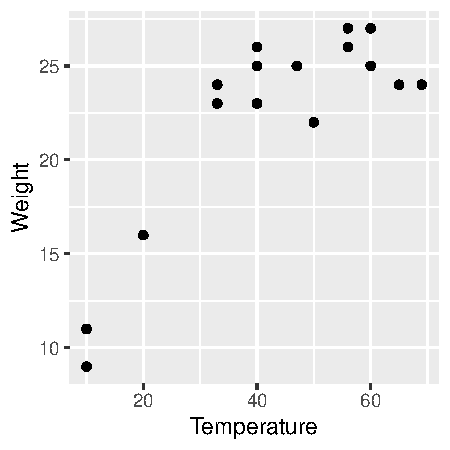
\includegraphics{modelquestions_files/figure-latex/unnamed-chunk-2-1.pdf}

\textbf{Output b}

\begin{verbatim}

Call:
lm(formula = Weight ~ Temperature, data = df)

Residuals:
    Min      1Q  Median      3Q     Max 
-5.2450 -2.0422  0.4882  1.6926  4.4071 

Coefficients:
            Estimate Std. Error t value Pr(>|t|)    
(Intercept) 11.79572    2.03828   5.787 3.58e-05 ***
Temperature  0.24493    0.04318   5.672 4.43e-05 ***
---
Signif. codes:  0 '***' 0.001 '**' 0.01 '*' 0.05 '.' 0.1 ' ' 1

Residual standard error: 3.123 on 15 degrees of freedom
Multiple R-squared:  0.682, Adjusted R-squared:  0.6608 
F-statistic: 32.18 on 1 and 15 DF,  p-value: 4.429e-05
\end{verbatim}

\textbf{Output c}

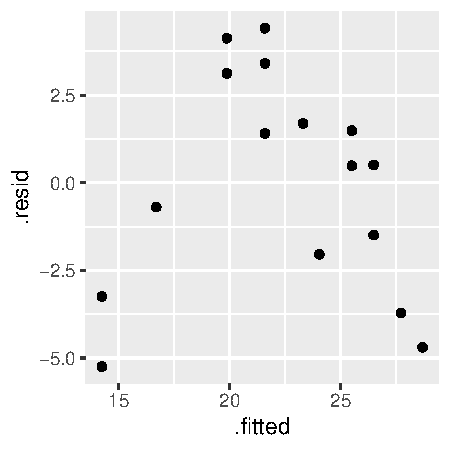
\includegraphics{modelquestions_files/figure-latex/unnamed-chunk-4-1.pdf}

\textbf{Output d}

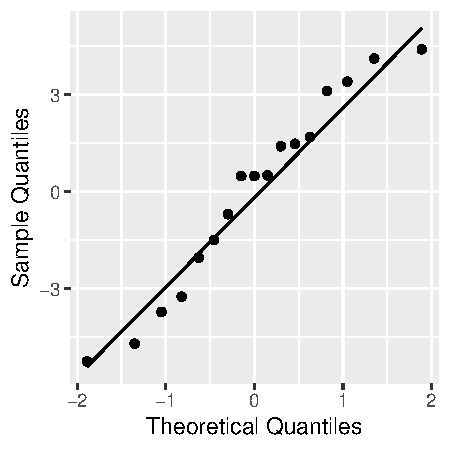
\includegraphics{modelquestions_files/figure-latex/unnamed-chunk-5-1.pdf}

\textbf{Output e}

\begin{verbatim}

    Shapiro-Wilk normality test

data:  fitmodel$.resid
W = 0.95278, p-value = 0.502
\end{verbatim}

\begin{enumerate}
\def\labelenumi{\roman{enumi})}
\setcounter{enumi}{1}
\tightlist
\item
  Two undergraduates studying statistics were looking at this analysis.
\end{enumerate}

\begin{enumerate}
\def\labelenumi{(\Alph{enumi})}
\item
  One said that the results strongly suggest that this model is highly
  significant and can be used for prediction purposes.
\item
  The other said that the results show the fitted model is not
  appropriate for this case and this model cannot be used for
  prediction.
\end{enumerate}

With whom would you agree? Justify your argument using each part ((a) to
(e)) of the results given.

\hypertarget{question-2}{%
\subsection{Question 2}\label{question-2}}

In a soap production factory, there are two machines used for the
production. Using 27 production runs; 15 of line 1 and 12 of line 2, the
management wanted to find the relationship between the machine speed and
the amount of scrap produced during the production process. To allow the
two machines have different regression lines with different intercepts
and slopes the following model was fitted with all 27 observations.

\[Y = \beta_0 + \beta_1 X_1 + \beta_2 X_2 + \beta_3 X_1 X_2 + \epsilon\]

where,

\(X_1\) is line speed and

\begin{equation}
  X_{2} =
  \begin{cases}
    1 & \text{if line 1} \\
    0 & \text{if line 2}
  \end{cases}
\end{equation}

\begin{enumerate}
\def\labelenumi{\roman{enumi})}
\item
  Draw a sketch of the scatter plot which is expected with the above
  model.
\item
  Write the model for each machine.
\item
  Write the hypotheses that should be tested to find whether the two
  machines have the same regression model or not, i.e.~whether both the
  intercept and the slope are the same of the two models you wrote in
  ii) in the above.
\end{enumerate}

\hypertarget{question-3}{%
\subsection{Question 3}\label{question-3}}

A group of new graduates who have studied Statistics, Mathematics and
Computer Science at the Faculty of Applied Sciences of University of
Jayewardenepura joined a company. They were given three tests in the
three subjects they have studied for the degree at the final interview
at which they were selected for the job. After three months of a
probationary period, their proficiency for the job was measured. The
tests scores and the measure of proficiency were analyzed to find a
model to predict proficiency by the test scores. Some results are shown
below.

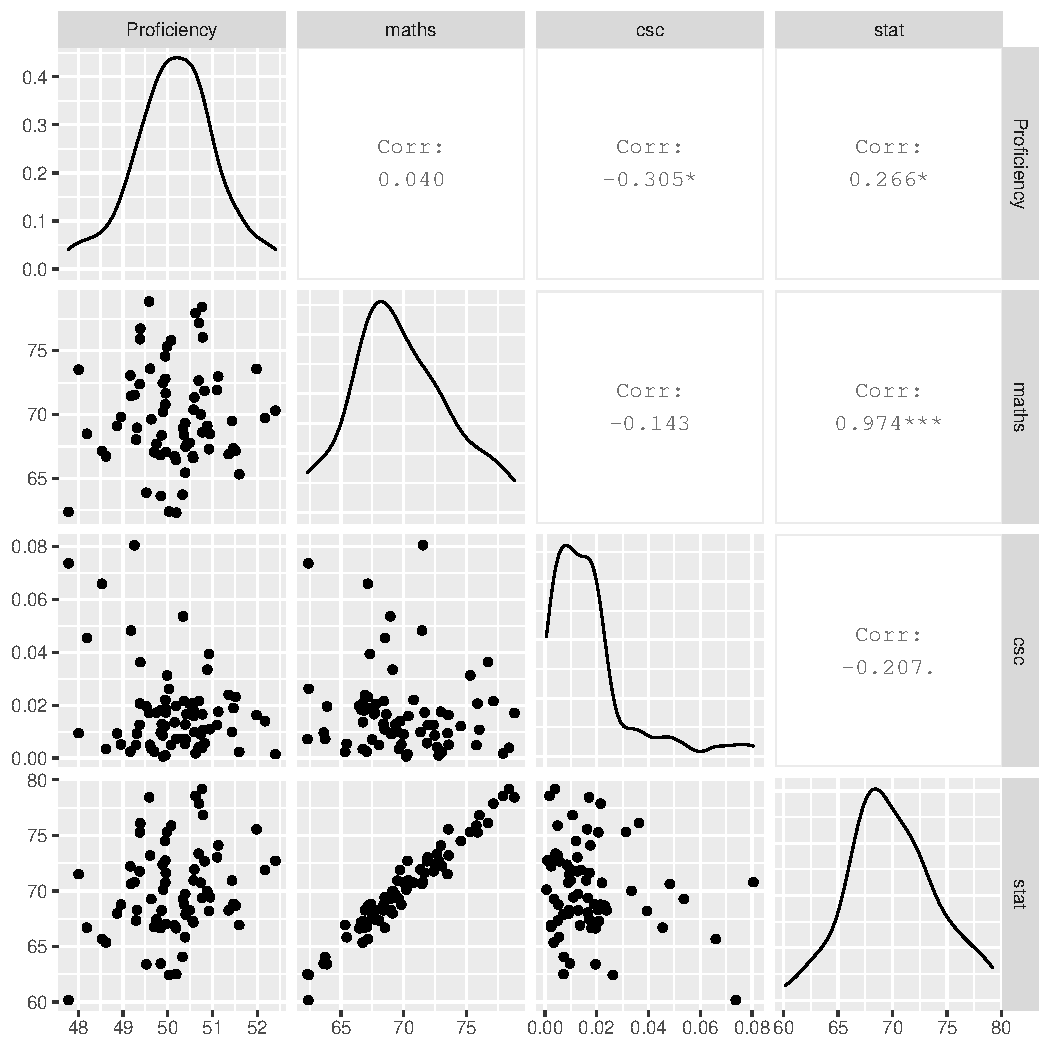
\includegraphics{modelquestions_files/figure-latex/unnamed-chunk-7-1.pdf}

\begin{Shaded}
\begin{Highlighting}[]
\NormalTok{model.sjp <-}\StringTok{ }\KeywordTok{lm}\NormalTok{(Proficiency }\OperatorTok{~}\StringTok{ }\NormalTok{maths }\OperatorTok{+}\StringTok{ }\NormalTok{csc }\OperatorTok{+}\StringTok{ }\NormalTok{stat, }\DataTypeTok{data=}\NormalTok{df)}
\KeywordTok{summary}\NormalTok{(model.sjp)}
\end{Highlighting}
\end{Shaded}

\begin{verbatim}

Call:
lm(formula = Proficiency ~ maths + csc + stat, data = df)

Residuals:
       Min         1Q     Median         3Q        Max 
-1.136e-13  5.390e-16  2.112e-15  2.632e-15  9.808e-15 

Coefficients:
              Estimate Std. Error    t value Pr(>|t|)    
(Intercept)  5.000e+01  3.311e-14  1.510e+15   <2e-16 ***
maths       -1.000e+00  2.113e-15 -4.732e+14   <2e-16 ***
csc          1.647e-14  1.175e-13  1.400e-01    0.889    
stat         1.000e+00  2.062e-15  4.849e+14   <2e-16 ***
---
Signif. codes:  0 '***' 0.001 '**' 0.01 '*' 0.05 '.' 0.1 ' ' 1

Residual standard error: 1.51e-14 on 66 degrees of freedom
Multiple R-squared:      1, Adjusted R-squared:      1 
F-statistic: 8.644e+28 on 3 and 66 DF,  p-value: < 2.2e-16
\end{verbatim}

\begin{Shaded}
\begin{Highlighting}[]
\NormalTok{car}\OperatorTok{::}\KeywordTok{vif}\NormalTok{(model.sjp)}
\end{Highlighting}
\end{Shaded}

\begin{verbatim}
    maths       csc      stat 
20.786453  1.123955 21.276288 
\end{verbatim}

A statistician examined these results and claimed that
``multicollinearity'' has affected this model.

\begin{enumerate}
\def\labelenumi{\roman{enumi})}
\item
  What is meant by multicollinearity?
\item
  Do you agree with statistician claim. Justify your answer.
\item
\end{enumerate}

\hypertarget{question-4}{%
\subsection{Question 4}\label{question-4}}

it is required to study the relationship between age (\(X\)) and girth
(\(Y\)) of teak trees growing in a plantation. Note that girth is the
diameter of the tree (in inches) measured at 5 inches above the ground.
The girth of the trees and the ages (in years) have been recorded from a
sample of 25 trees. Assume that the scatterplot of the data clearly
shows a linear relationship between the two variables with an intercept.

\begin{enumerate}
\def\labelenumi{\roman{enumi})}
\item
  Write the simple linear regression model that you would be fitted for
  the above variables. Define all terms in it and state any assumptions
  regarding the model.
\item
  Later it was suggested that a linear model goes through the origin is
  suitable for this situation. Write the new model using the usual
  notation.
\item
  The estimated regression model in part (ii) satisfied all of the
  assumptions regarding the error term. Sketch the residual plot vs
  fitted values and Q-Q normality plot of residuals.
\end{enumerate}

\hypertarget{question-5}{%
\subsection{Question 5}\label{question-5}}

An experiment was conducted to determine the influence of sulfide
concentration (\(X_1\)) on the whiteness of rayon (\(Y\)). The results
obtained through R are given below.

\begin{Shaded}
\begin{Highlighting}[]
\NormalTok{x1 <-}\StringTok{ }\KeywordTok{rnorm}\NormalTok{(}\DecValTok{15}\NormalTok{, }\DataTypeTok{mean=}\DecValTok{40}\NormalTok{)}
\NormalTok{y <-}\StringTok{ }\DecValTok{13} \OperatorTok{+}\StringTok{ }\NormalTok{(}\DecValTok{2}\OperatorTok{*}\NormalTok{x1) }\OperatorTok{+}\StringTok{ }\KeywordTok{rnorm}\NormalTok{(}\DecValTok{15}\NormalTok{)}
\NormalTok{df5 <-}\StringTok{ }\KeywordTok{data.frame}\NormalTok{(}\DataTypeTok{x1=}\NormalTok{x1, }\DataTypeTok{Y=}\NormalTok{y)}
\NormalTok{mod5 <-}\StringTok{ }\KeywordTok{lm}\NormalTok{(Y }\OperatorTok{~}\StringTok{ }\NormalTok{x1, }\DataTypeTok{data=}\NormalTok{df5)}
\KeywordTok{summary}\NormalTok{(mod5)}
\end{Highlighting}
\end{Shaded}

\begin{verbatim}

Call:
lm(formula = Y ~ x1, data = df5)

Residuals:
     Min       1Q   Median       3Q      Max 
-1.69929 -0.48179  0.02163  0.66530  1.31226 

Coefficients:
            Estimate Std. Error t value Pr(>|t|)    
(Intercept)   21.718     12.780   1.699    0.113    
x1             1.786      0.321   5.563 9.19e-05 ***
---
Signif. codes:  0 '***' 0.001 '**' 0.01 '*' 0.05 '.' 0.1 ' ' 1

Residual standard error: 0.9087 on 13 degrees of freedom
Multiple R-squared:  0.7042,    Adjusted R-squared:  0.6814 
F-statistic: 30.94 on 1 and 13 DF,  p-value: 9.185e-05
\end{verbatim}

\begin{Shaded}
\begin{Highlighting}[]
\KeywordTok{anova}\NormalTok{(mod5)}
\end{Highlighting}
\end{Shaded}

\begin{verbatim}
Analysis of Variance Table

Response: Y
          Df Sum Sq Mean Sq F value    Pr(>F)    
x1         1 25.550 25.5497  30.944 9.185e-05 ***
Residuals 13 10.734  0.8257                      
---
Signif. codes:  0 '***' 0.001 '**' 0.01 '*' 0.05 '.' 0.1 ' ' 1
\end{verbatim}

\begin{enumerate}
\def\labelenumi{\roman{enumi})}
\item
  Construct the ANOVA table using the above results.
\item
  Wtite the hypothesis to be tested in the ANOVA in part i.
\item
  What is your decision about the fitted model.
\end{enumerate}

\end{document}
